\documentclass[11pt,a4paper,fontset=none]{ctexart}
\setCJKmainfont[Path=/System/Library/Fonts/Supplemental/]{Songti.ttc}
\setCJKsansfont[Path=/System/Library/Fonts/]{Hiragino Sans GB.ttc}
\usepackage[margin=2.35cm]{geometry}
\usepackage{amsmath,booktabs,graphicx,array,float,hyperref}
\usepackage[table]{xcolor}
\hypersetup{colorlinks=true,linkcolor=blue,urlcolor=blue}
\setlength{\parindent}{2em}
\setlength{\parskip}{0.25em}
\newcommand{\param}[1]{\texttt{\detokenize{#1}}}
\title{Assignment 2\\参数扰动方案与实验记录}
\author{Mathematical Methods in Uncertainty Quantification}
\date{持续更新}
\begin{document}
\maketitle

\section{模型和基准}
使用课程目录中 Assignment 1 的 HBV001a 模型、原校准范围以及校准结果文件中保存的最佳参数。评价沿用 Assignment 1 的设置：\(J=1-\mathrm{NSE}\)，无预热期。基准模型复现结果为
\[
J^*=0.0927763,\qquad \mathrm{NSE}^*=0.907224.
\]
原校准范围作为硬限制。每次扰动均以这组参数为基准；若改用其他随机种子得到的参数组，需要重新核对可行范围。

\section{参数扰动的分类和处理}
本次对 Assignment 1 的 18 个校准量全部进行逐一扰动。参数的数值小并不意味着它不敏感，例如 \param{lrr_dre} 的校准值约为 0.00913，在本次实验中排名第三。参数具有不同单位和物理含义，不能仅凭数值大小排除。

\subsection{可以直接采用相对扰动的参数}
以下 12 个参数乘以 0.8 和 1.2 均在原校准范围内：\param{snw_att}、\param{snw_pmf}、\param{snw_amf}、\param{sl0_bt0}、\param{urr_dth}、\param{lrr_dth}、\param{urr_ulc}、\param{urr_tdh}、\param{urr_tdr}、\param{urr_ndr}、\param{urr_uct}、\param{lrr_lct}。

\subsection{受校准范围限制的参数}
每侧最多变化 20\%；若先碰到校准边界，就在边界停止。下表标注实际变化，受限方向的端点不是 20\%。
\begin{center}\small
\begin{tabular}{lrrrr}\toprule
参数 & 校准值约为 & 校准范围 & 较小方向 & 较大方向\\\midrule
\param{snw_dth} & 8.58808 & 0--10 & $-20\%$ & $+16.44\%$\\
\param{sl0_dth} & 49.06446 & 0--50 & $-20\%$ & $+1.91\%$\\
\param{sl0_pwp} & 646.54862 & 5--700 & $-20\%$ & $+8.27\%$\\
\param{sl0_fcy} & 122.27323 & 100--700 & $-18.22\%$ & $+20\%$\\
\param{urr_wsr} & 0.99104 & 0--1 & $-20\%$ & $+0.90\%$\\
\param{lrr_dre} & 0.00913049 & 0--0.01 & $-20\%$ & $+9.52\%$\\\bottomrule
\end{tabular}
\end{center}
不同参数的可行范围不完全相同；其中 \param{sl0_dth} 和 \param{urr_wsr} 的正向范围尤其窄。

\subsection{温度阈值的说明}
\param{snw_att} 的基准值约为 $-0.00604556\,^\circ\mathrm{C}$。本次同样乘以 0.8 和 1.2，对应温度约 $-0.00483645$ 和 $-0.00725467\,^\circ\mathrm{C}$，与基准相差约 $0.00120911\,^\circ\mathrm{C}$。由于基准为负，乘以 1.2 使实际温度降低；摄氏温标的零点也使百分比扰动需要谨慎解释。本次未测试更大的绝对温度变化。

\section{单参数局部敏感性实验}
每次只改变一个参数，其余均保持基准值。每个参数在基准两侧各取 10 个等距点，加上基准共 21 点；18 个参数合计记录 378 点。目标函数变化和排名指标分别为
\[
\Delta J(\%)=100\frac{J(\theta_i')-J^*}{J^*},\qquad S_i=\frac{1}{20}\sum_{k=1}^{20}|\Delta J_{i,k}(\%)|.
\]
\(S_i\) 为 20 个非基准点的平均绝对目标函数变化。不同参数的可行范围不同，排名不是完全等扰动条件下的比较。
\begin{center}\small
\begin{tabular}{rlrr}\toprule
排名 & 参数 & 平均绝对变化 & 相对扰动范围\\\midrule
1 & \param{sl0_fcy} & 5.8126\% & $-18.22\%$ 至 $+20.00\%$\\
2 & \param{snw_pmf} & 4.7719\% & $-20.00\%$ 至 $+20.00\%$\\
3 & \param{lrr_dre} & 4.2247\% & $-20.00\%$ 至 $+9.52\%$\\
4 & \param{sl0_bt0} & 0.70836\% & $-20.00\%$ 至 $+20.00\%$\\
5 & \param{sl0_dth} & 0.6923\% & $-20.00\%$ 至 $+1.91\%$\\
6 & \param{snw_amf} & 0.49607\% & $-20.00\%$ 至 $+20.00\%$\\
7 & \param{snw_att} & 0.36891\% & $-20.00\%$ 至 $+20.00\%$\\
8 & \param{urr_ulc} & 0.33188\% & $-20.00\%$ 至 $+20.00\%$\\
9 & \param{urr_wsr} & 0.10211\% & $-20.00\%$ 至 $+0.90\%$\\
10 & \param{snw_dth} & 0.040245\% & $-20.00\%$ 至 $+16.44\%$\\
11 & \param{sl0_pwp} & 0.0048632\% & $-20.00\%$ 至 $+8.27\%$\\
12 & \param{lrr_dth} & 0.0034587\% & $-20.00\%$ 至 $+20.00\%$\\
13 & \param{lrr_lct} & 0.0026344\% & $-20.00\%$ 至 $+20.00\%$\\
14 & \param{urr_uct} & 0.0014379\% & $-20.00\%$ 至 $+20.00\%$\\
15 & \param{urr_dth} & 0.00095492\% & $-20.00\%$ 至 $+20.00\%$\\
16 & \param{urr_ndr} & 0.00075207\% & $-20.00\%$ 至 $+20.00\%$\\
17（并列） & \param{urr_tdh} & 0\% & $-20.00\%$ 至 $+20.00\%$\\
17（并列） & \param{urr_tdr} & 0\% & $-20.00\%$ 至 $+20.00\%$\\
\bottomrule
\end{tabular}
\end{center}
\param{snw_att} 的平均绝对变化约为 0.369\%，表明本次测试出现了目标函数变化；这只反映上述极小的相对扰动，不能据此推断更大绝对温度变化的影响。\param{urr_tdh} 和 \param{urr_tdr} 在本次测试点没有使目标函数变化，不代表其他条件下也如此。

\section{排名前三参数的作用路径}
目标函数将各时间步模拟流量与观测流量的误差平方后加总。参数扰动改变误差的大小和时间分布，从而改变整个时段的目标函数。前三个参数在本次测试的两个端点都使 \(J\) 增大。

\subsection{\param{sl0_fcy}：土壤最大含水容量}
它影响土壤储水空间及输入水分形成产流的比例，改变进入水库的水量与时间，进而影响模拟流量及目标函数。
\subsection{\param{snw_pmf}：降水引起的融雪系数}
它在有积雪、有降水且气温高于阈值时控制降水引起的融雪。扰动可能改变融雪水进入土壤的数量与时间，进而影响流量；总融雪还受剩余积雪和气温融雪限制。
\subsection{\param{lrr_dre}：下层水库河道出流系数}
它影响下层水库放水的快慢。增大时，当前储量中的水通常释放得更快，同时留给后续时刻的水减少，可能改变流量过程线。

以上解释依据模型方程；具体哪些时段或流量特征造成目标函数变化，仍需检查流量过程线。

\section{不敏感参数的初步分析}
\param{urr_tdh} 和 \param{urr_tdr} 控制上层水库快速出口的阈值与出流系数。基准模拟中，出口计算前上层储量最大约 18.12 mm，低于本次测试的最低阈值约 78.79 mm；该过程未触发，故两者在本次范围内不改变目标函数。

\param{urr_ndr} 控制的常规出口水量很小，基准期内约 0.009 mm；上下层地下水输出分别约 0.034 和 0.065 mm，且不直接计入校准河道流量，因此 \param{urr_uct}、\param{lrr_lct} 的影响也较小。\param{urr_dth} 和 \param{lrr_dth} 只直接设定初始储量，其影响可能随时间减弱，仍需过程线验证。\param{sl0_pwp} 控制蒸散发限制；基准实际蒸散发累计约 3.35 mm，相对于降水累计约 299.20 mm 较小，这为其影响较小提供了可能解释。

\section{前三名参数的组合扰动}
此前实验对 \param{sl0_fcy}、\param{snw_pmf}、\param{lrr_dre} 进行了 12 个两参数及 8 个三参数端点组合。当前三者重新纳入扰动且仍为前三，基准、端点及模型均未改变，因此此前的组合模拟仍适用，结果已重新核算。

三个参数的负端和正端依次为：\param{sl0_fcy} $-18.22\%$、$+20\%$；\param{snw_pmf} $-20\%$、$+20\%$；\param{lrr_dre} $-20\%$、$+9.52\%$。下表为联合扰动的 \(J\) 相对变化，符号顺序与参数顺序一致。
\begin{center}\small
\begin{tabular}{lrrrr}\toprule
参数组合 & $-/-$ & $-/+$ & $+/-$ & $+/+$\\\midrule
\param{sl0_fcy} / \param{snw_pmf} & 26.75\% & 25.24\% & 31.20\% & 25.78\%\\
\param{sl0_fcy} / \param{lrr_dre} & 20.09\% & 23.05\% & 49.52\% & 12.48\%\\
\param{snw_pmf} / \param{lrr_dre} & 34.86\% & 16.29\% & 29.52\% & 12.83\%\\\bottomrule
\end{tabular}
\end{center}
三个参数顺序为 \param{sl0_fcy} / \param{snw_pmf} / \param{lrr_dre}：
\begin{center}\small
\begin{tabular}{lrlr}\toprule
方向 & \(J\) 的变化 & 方向 & \(J\) 的变化\\\midrule
$-/-/-$ & 34.06\% & $+/-/-$ & 64.92\%\\
$-/-/+$ & 34.62\% & $+/-/+$ & 26.13\%\\
$-/+/-$ & 32.13\% & $+/+/-$ & 58.82\%\\
$-/+/+$ & 34.67\% & $+/+/+$ & 22.08\%\\\bottomrule
\end{tabular}
\end{center}
\param{sl0_fcy} 和 \param{lrr_dre} 均取正端时，单独影响分别为 16.47\% 和 2.92\%，简单相加为 19.38\%，联合变化为 12.48\%，体现部分抵消。三个参数都取正端时，单独影响之和为 29.13\%，联合变化为 22.08\%。三个参数的联合偏离包括两两及更高阶作用；20 个端点组合没有完全回到基准，但不排除中间幅度有更强抵消。

\clearpage
\section{扰动曲线和敏感性排名图}
图中每个点表示一个参数扰动，其他参数保持基准。横轴是参数相对变化，纵轴是目标函数相对变化；温度阈值为负，横轴上的正百分比表示其温度值更负。各参数可行范围不同，曲线的横轴范围不一定对称。
\begin{figure}[H]
\centering
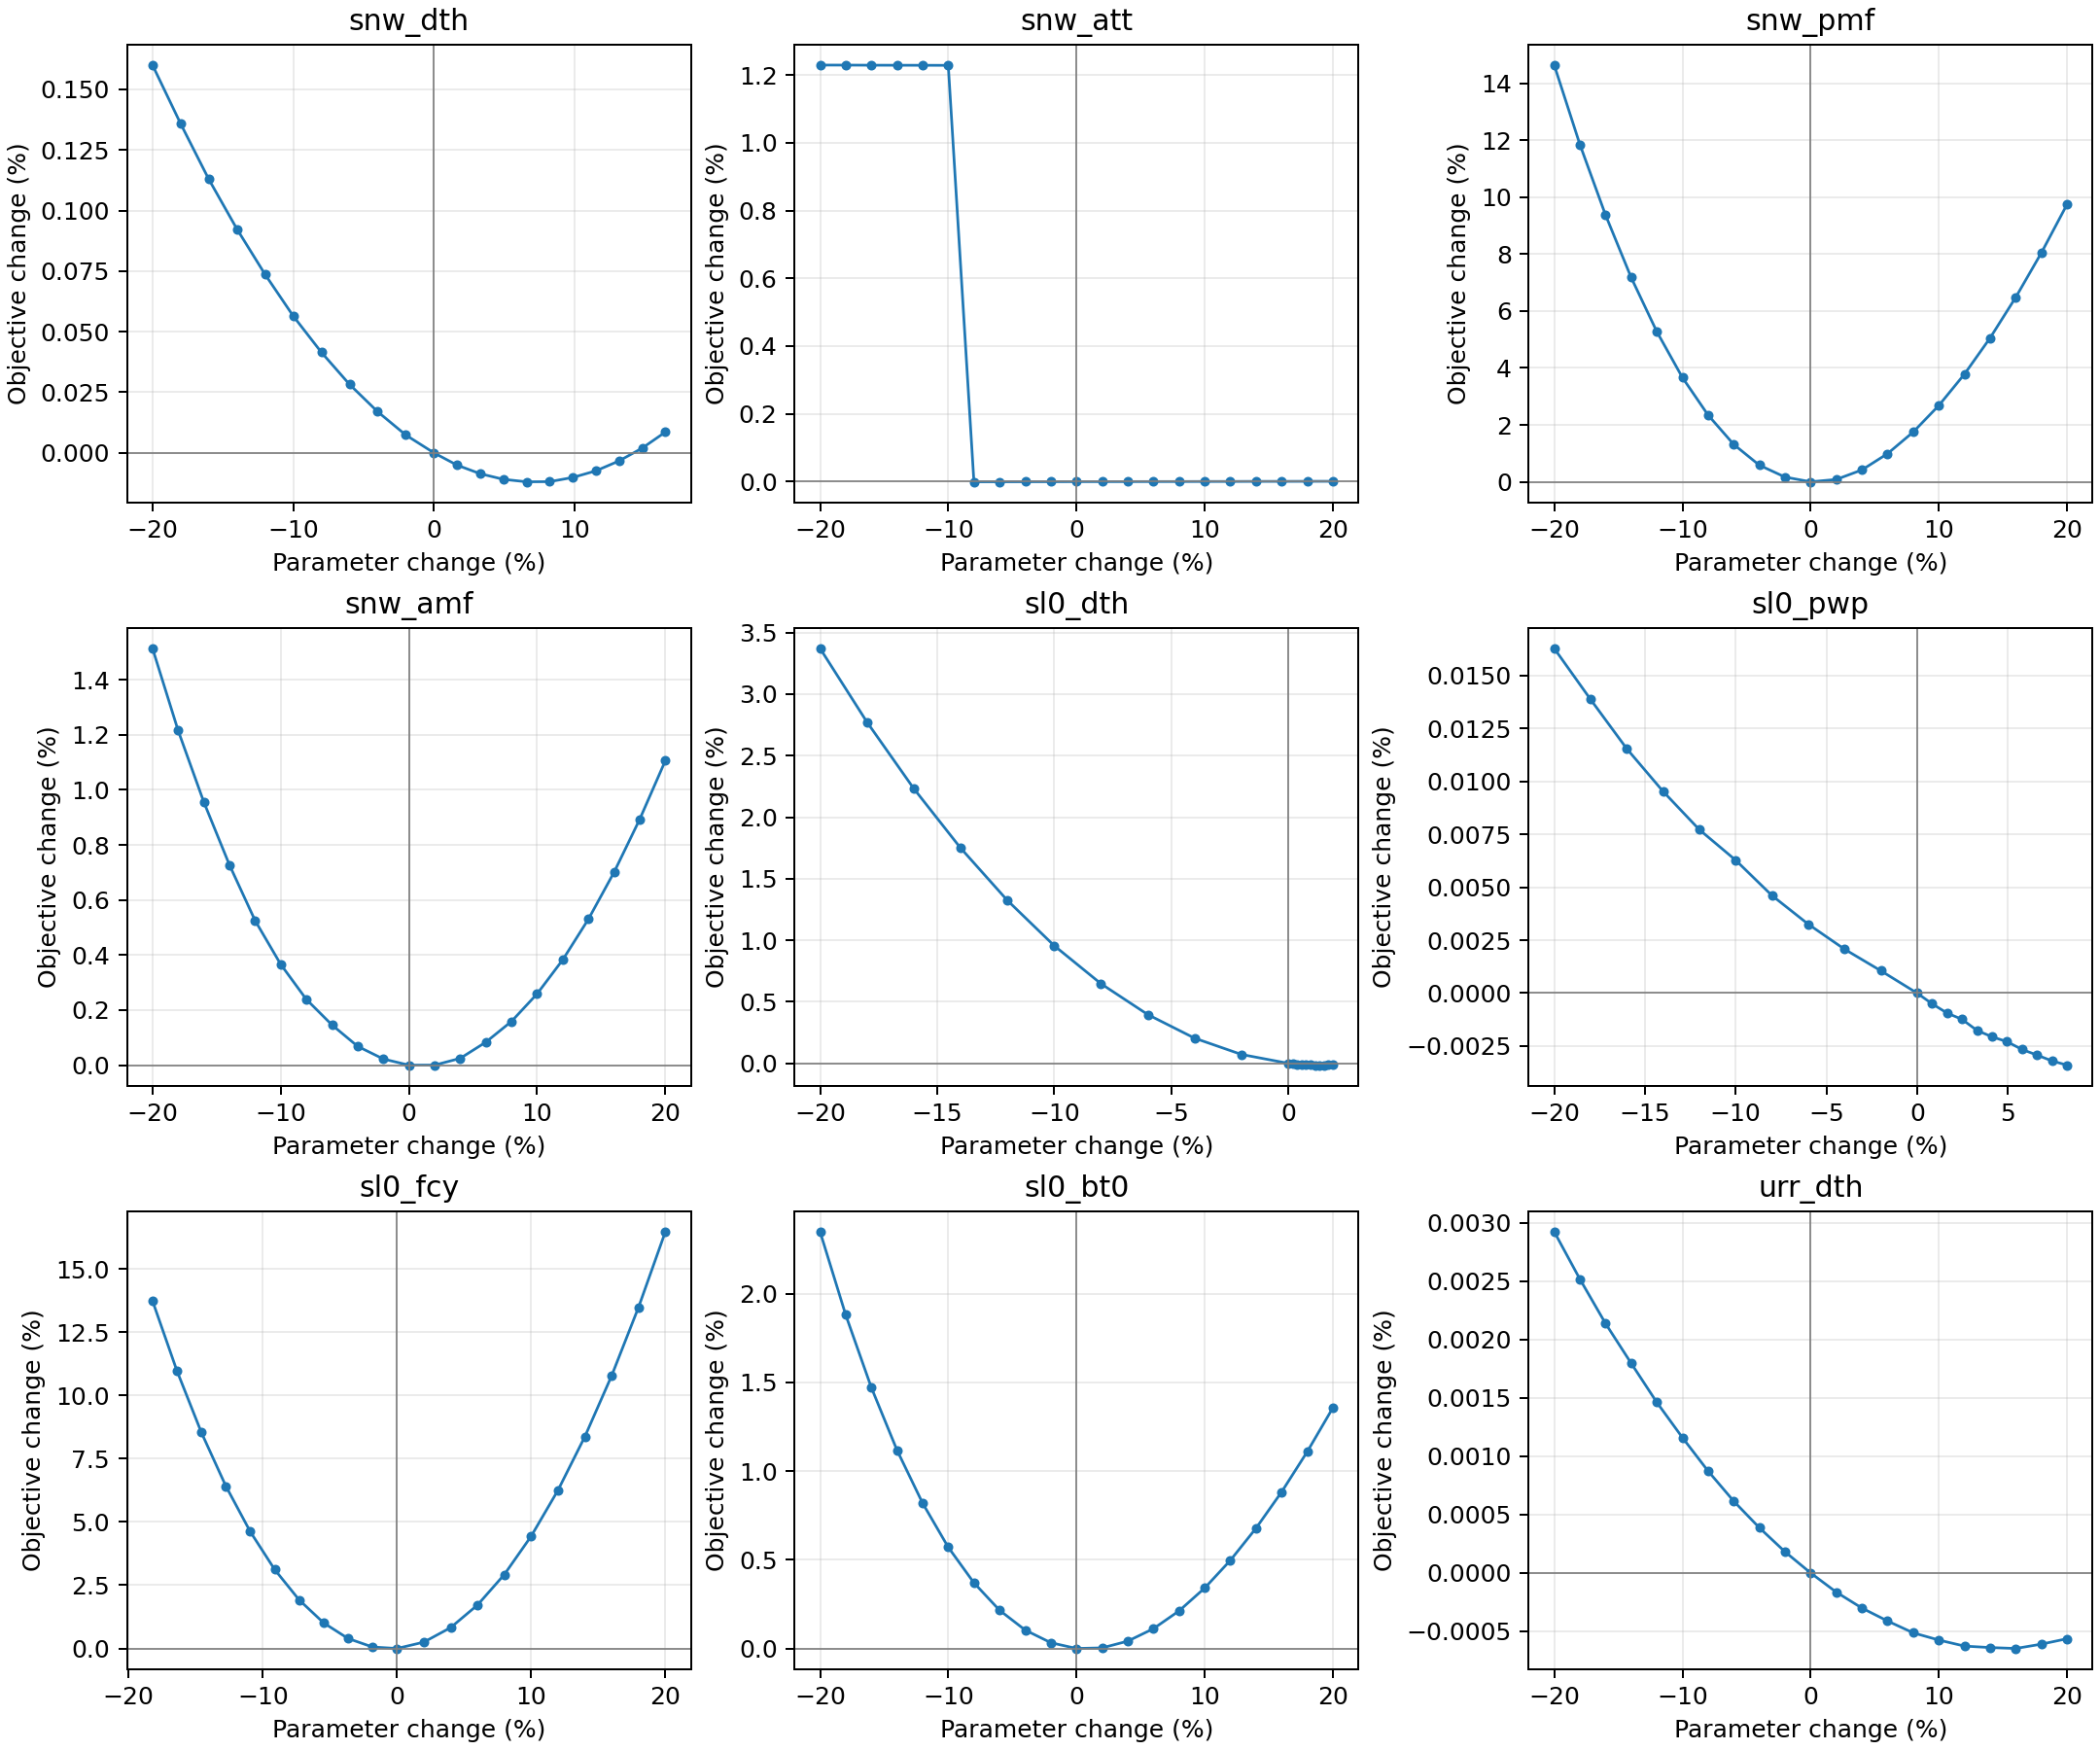
\includegraphics[width=\textwidth]{figures/perturbation_curves_1.png}
\caption{单参数扰动曲线，前 9 个参数。}
\end{figure}
\begin{figure}[H]
\centering
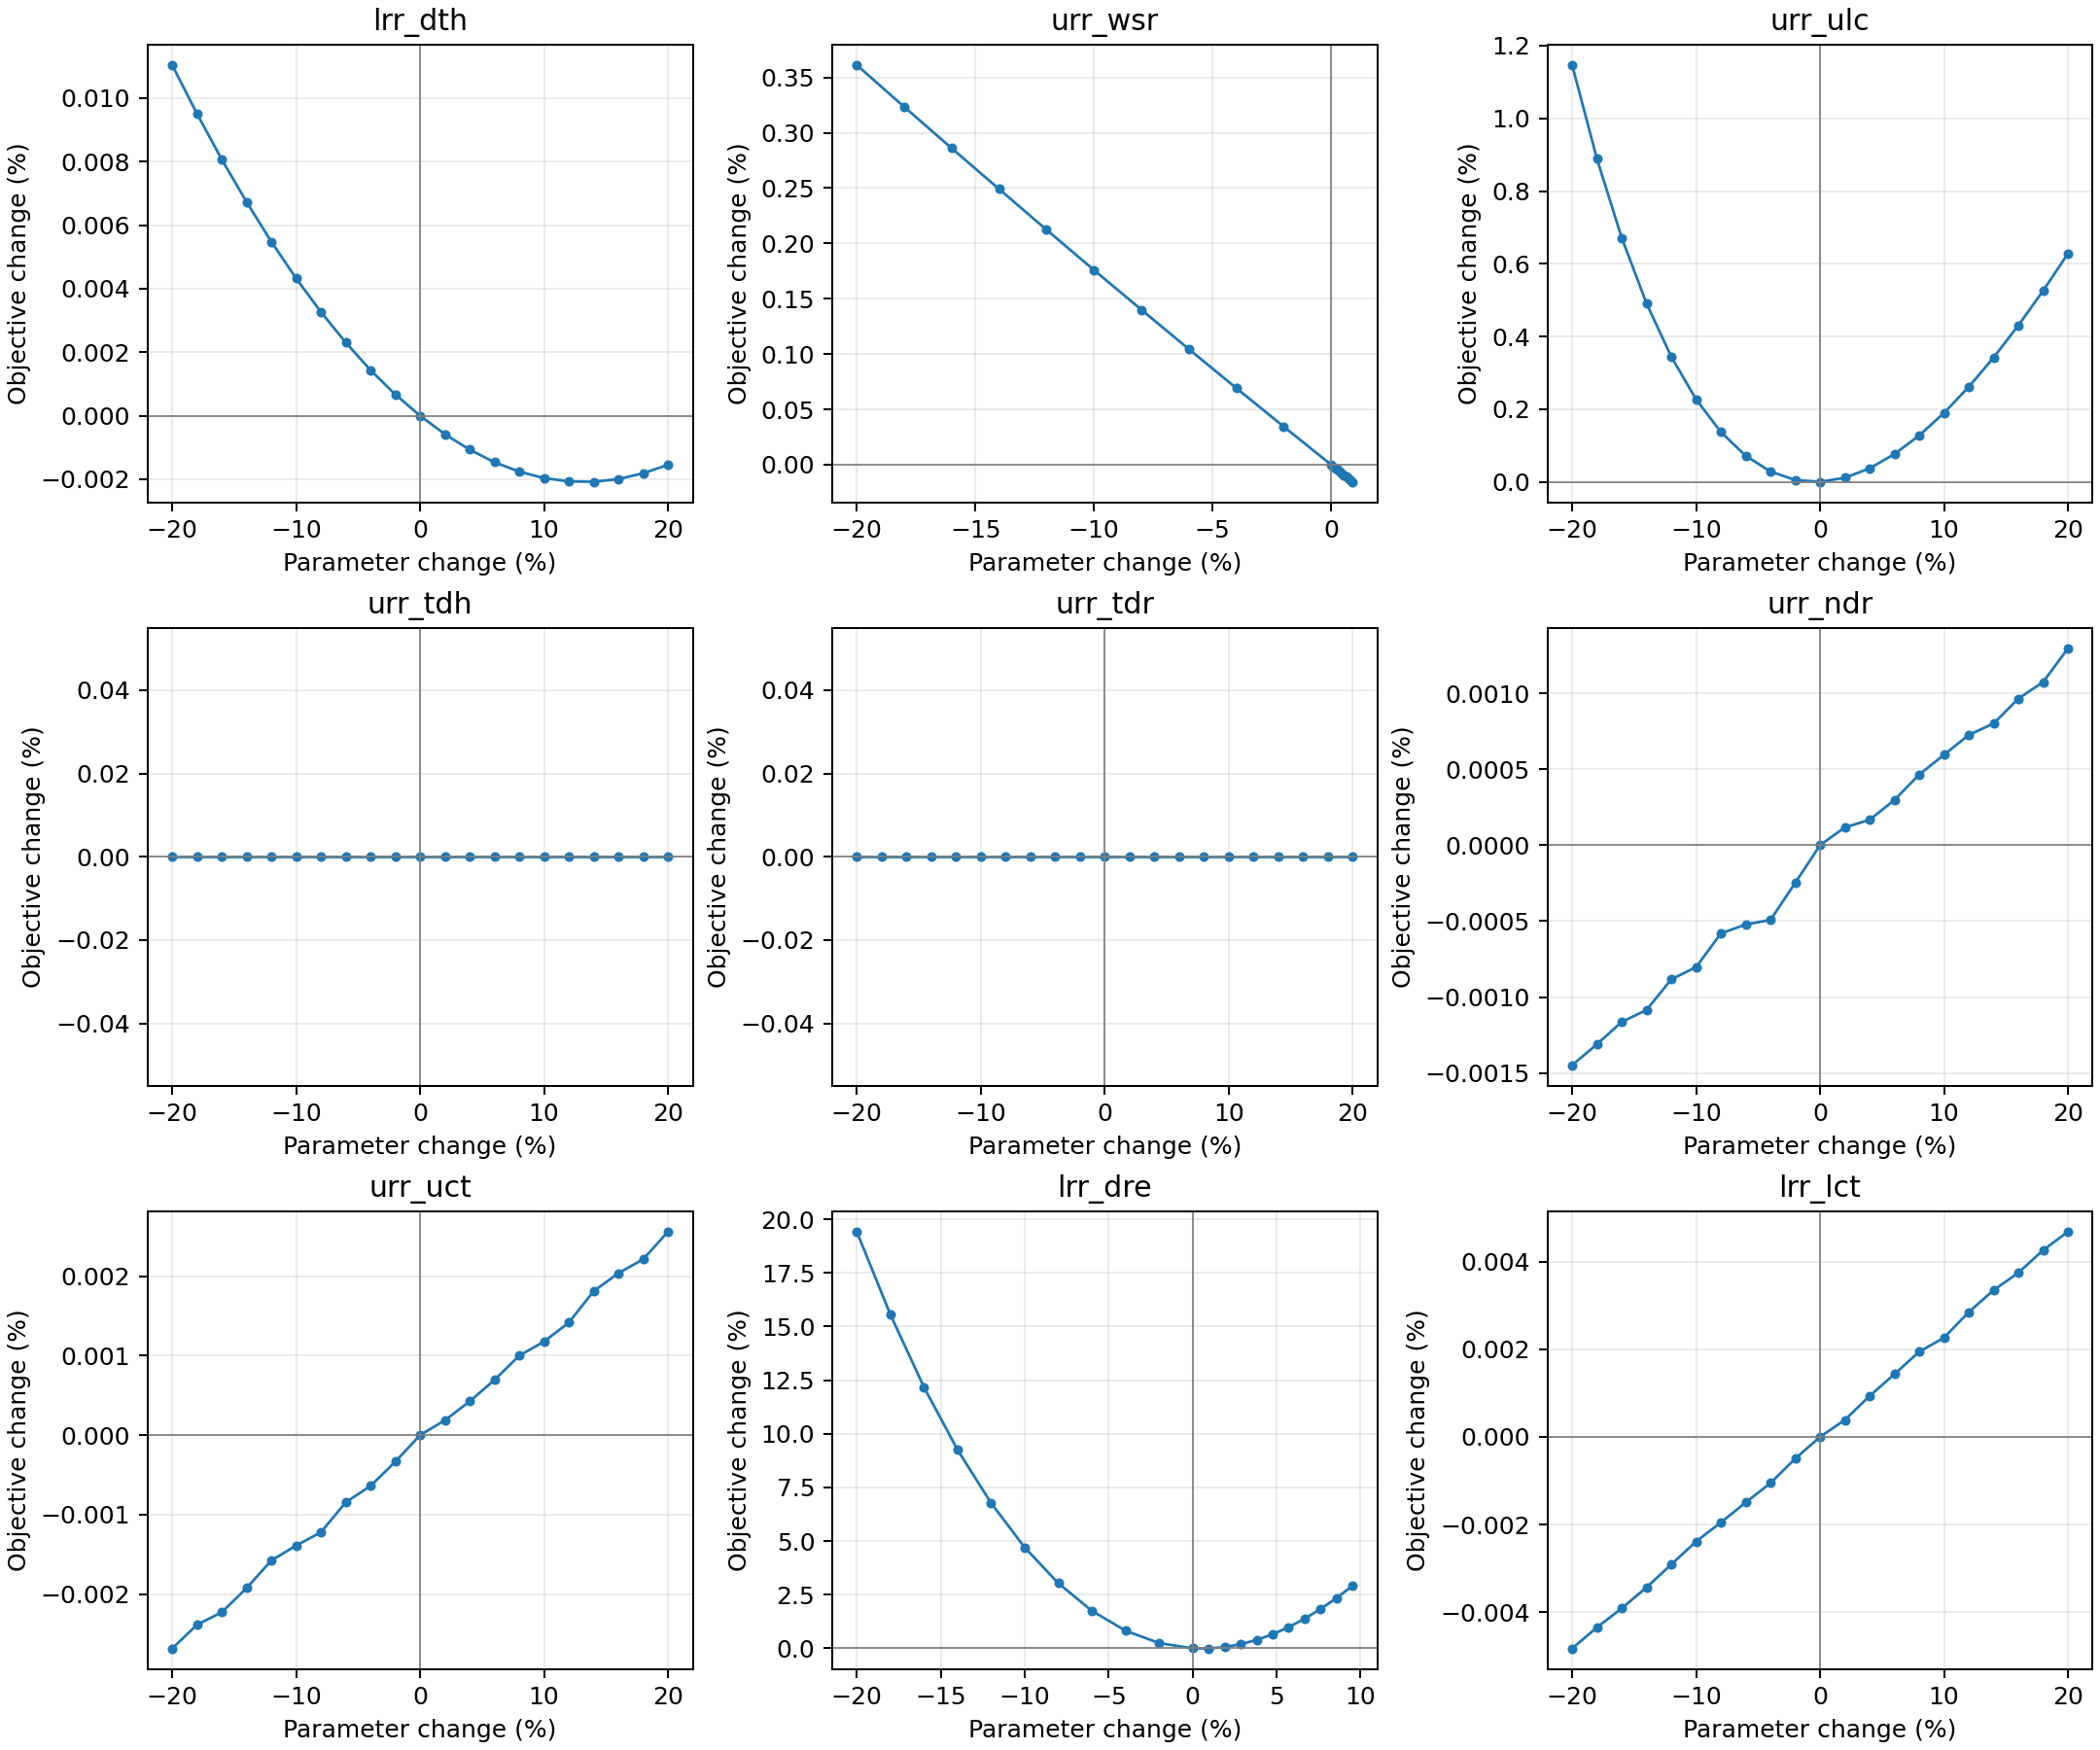
\includegraphics[width=\textwidth]{figures/perturbation_curves_2.png}
\caption{单参数扰动曲线，后 9 个参数。}
\end{figure}
\begin{figure}[H]
\centering
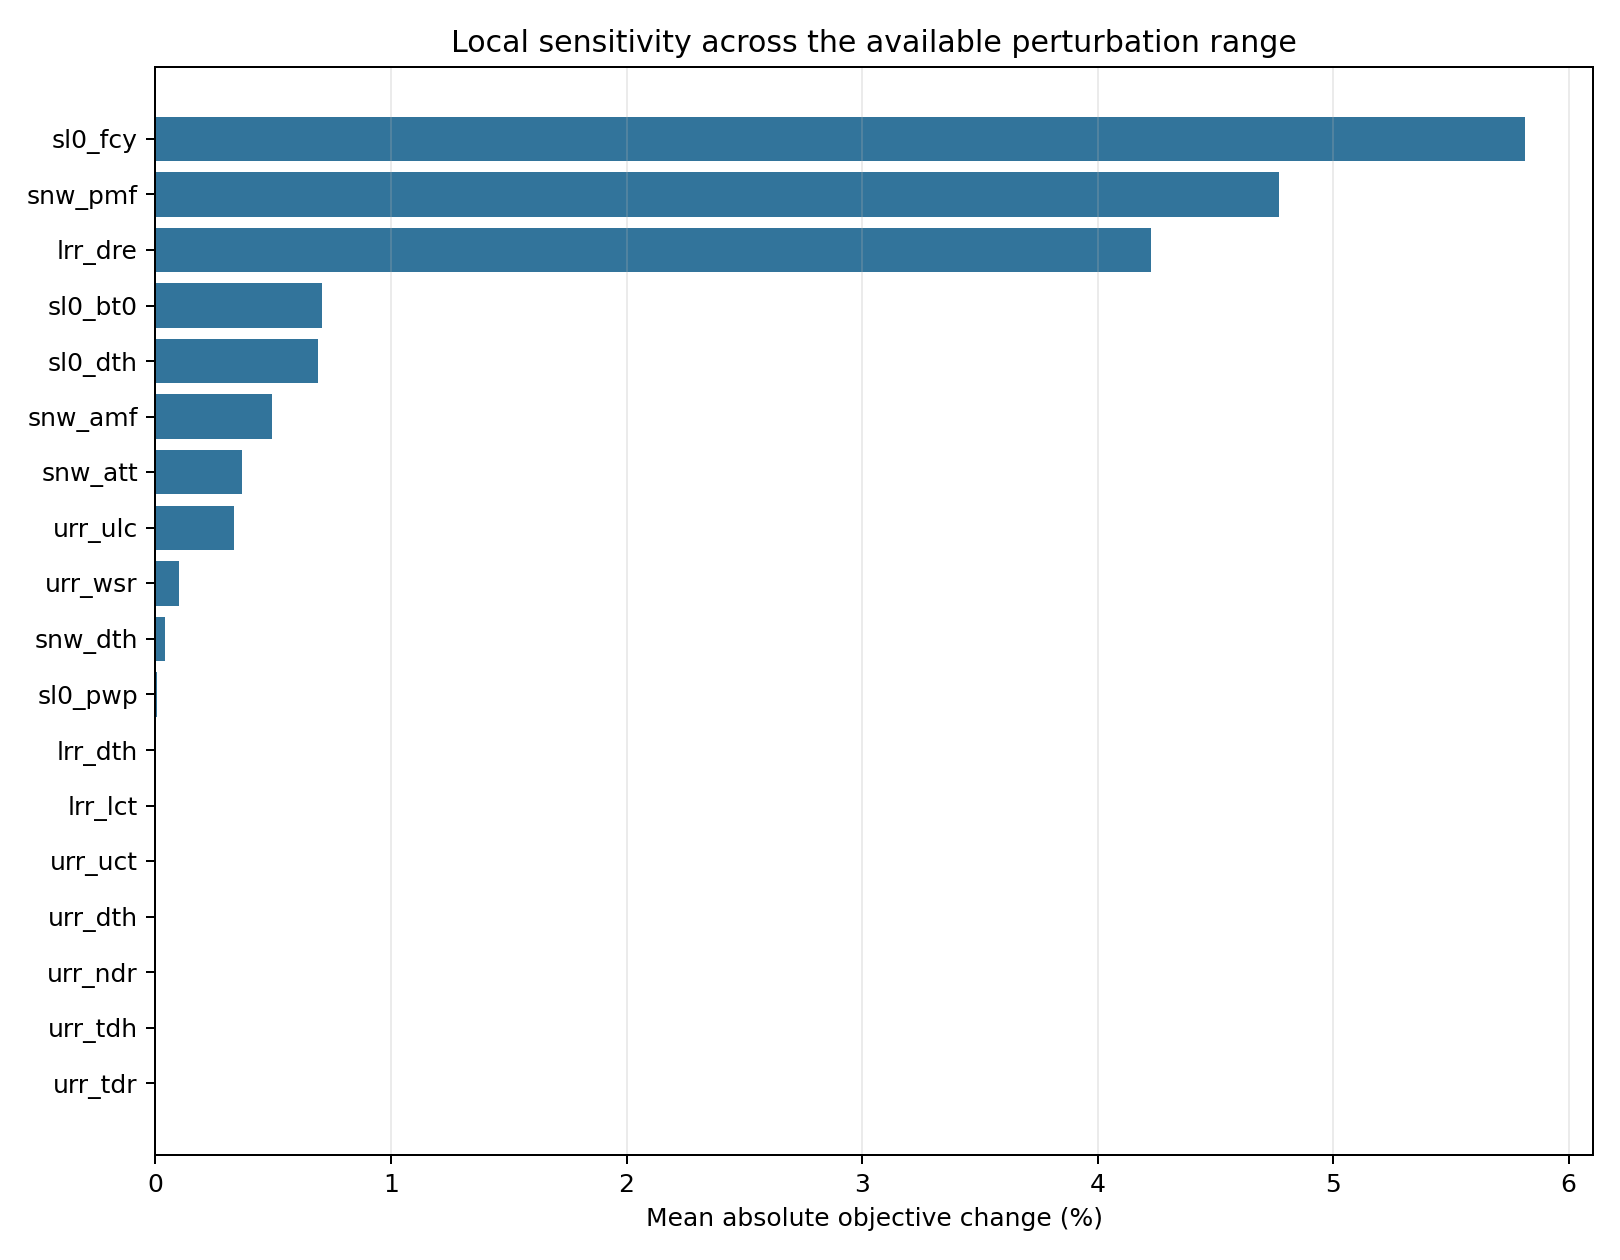
\includegraphics[width=0.93\textwidth]{figures/sensitivity_ranking.png}
\caption{按各自可行范围内目标函数平均绝对变化计算的排名。}
\end{figure}

\clearpage
\section{前三名参数的流量过程线对比}
每幅图比较观测流量、基准模拟流量和该参数两端扰动的模拟流量，其他参数固定。上图为完整时间序列，下图是一个 72 小时诊断窗口。窗口选择方法：计算两个端点在每小时相对基准的平方误差变化，取两个端点绝对变化之和最大的连续 72 小时。这个窗口用于展示较明显的变化，并不自动代表它对目标函数的净贡献最大。

图例中的参数变化为实际相对变化，括号是该端点在整个时间序列上的目标函数变化。对任一小时，平方误差变化可以为正或负；各时段可能相互抵消，因此不能仅凭流量曲线的间距判断对整个目标函数的净影响。

\begin{figure}[H]
\centering
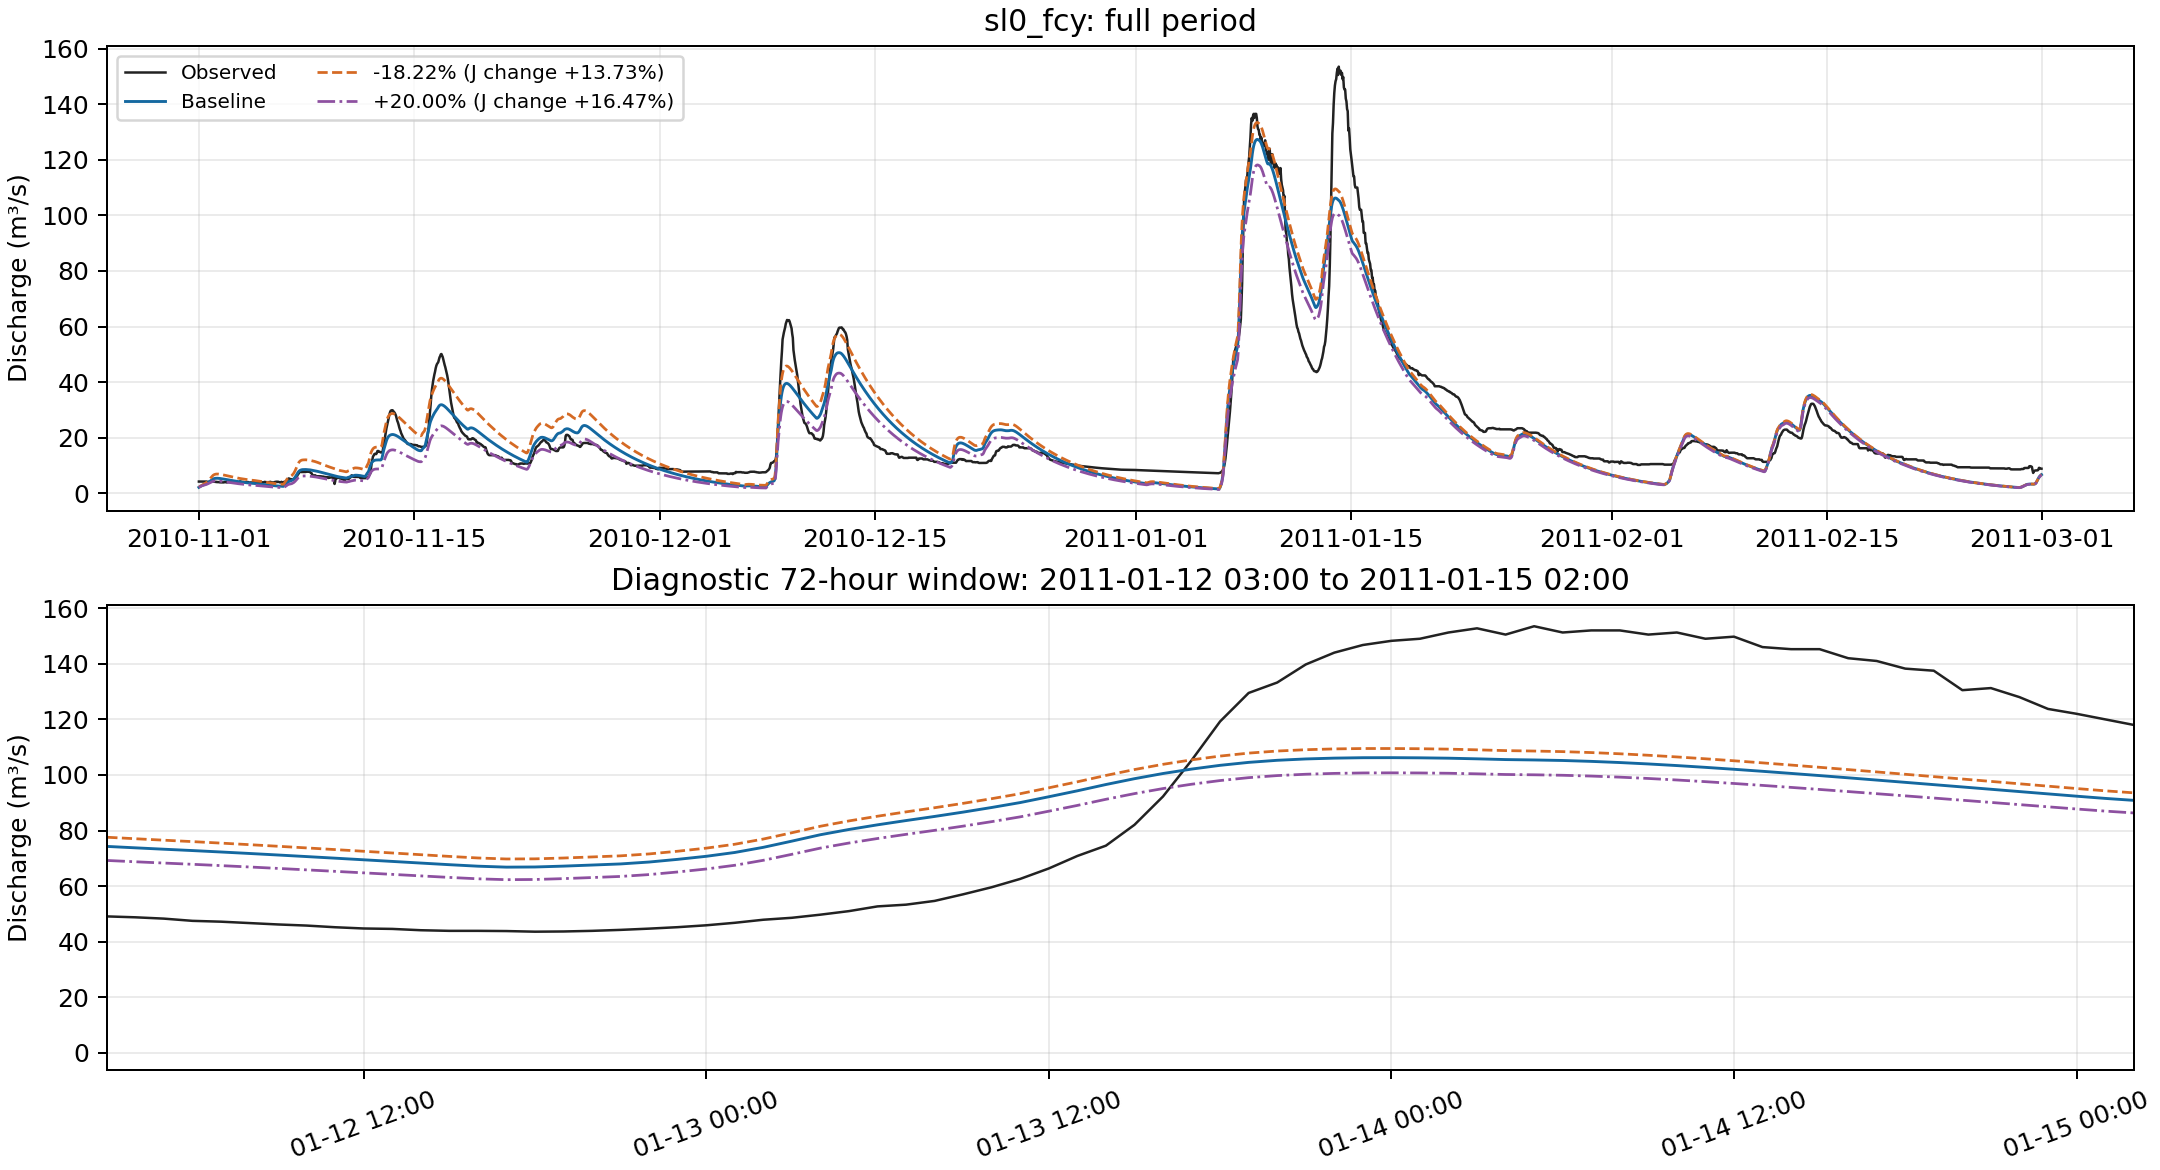
\includegraphics[width=\textwidth]{figures/hydrograph_sl0_fcy.png}
\caption{土壤最大含水容量的流量响应。}
\end{figure}
\param{sl0_fcy} 的诊断窗口为 2011 年 1 月 12--15 日。该窗口中，正端扰动使平方误差的净增加量约占全时段净增加量的 20.9\%；负端在这一窗口反而使误差净减少，但全时段目标函数仍增加。可见不同时间段的影响方向并不一定相同。

\begin{figure}[H]
\centering
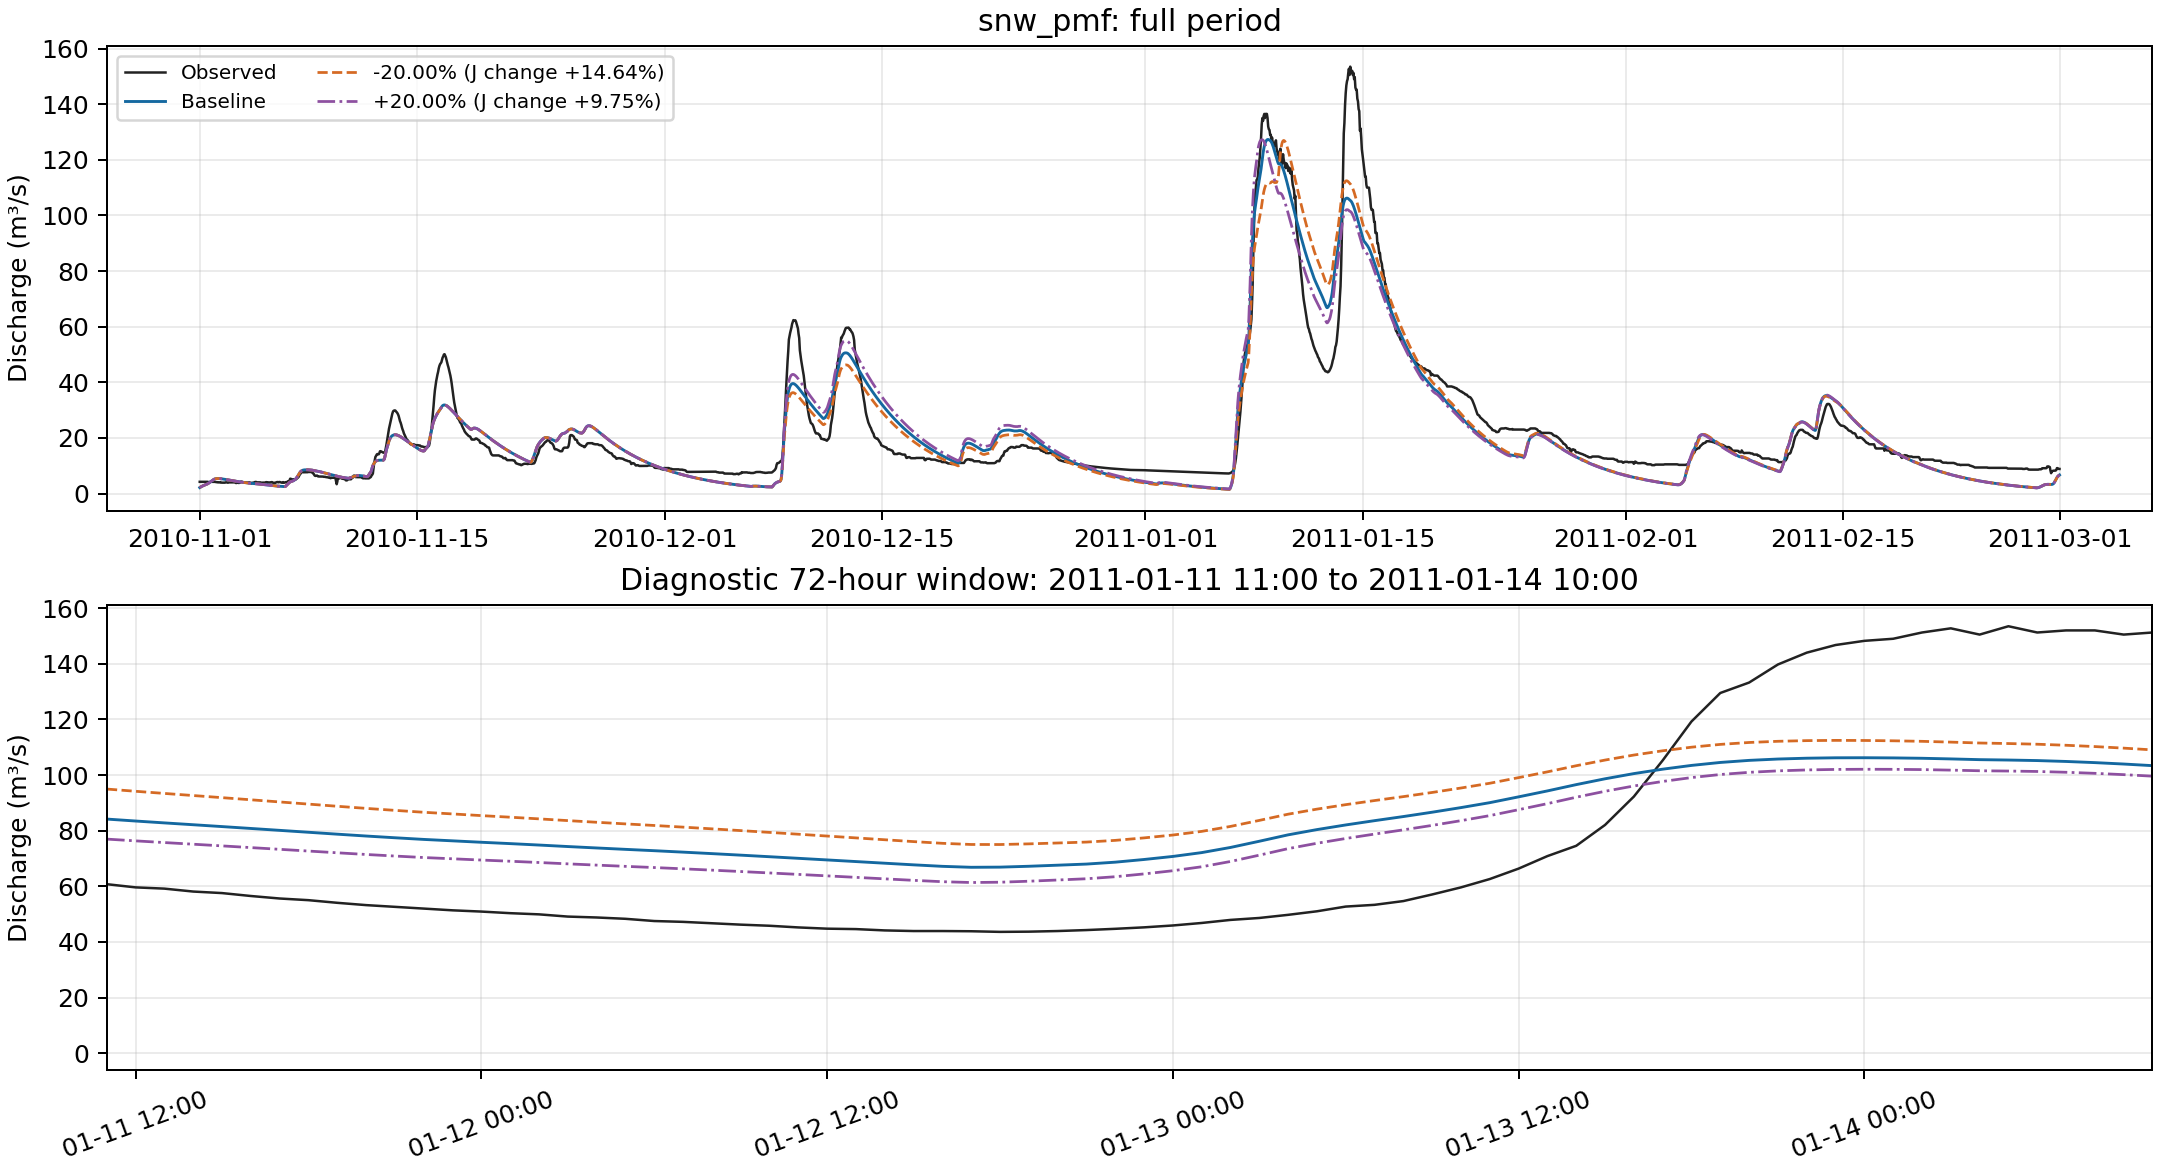
\includegraphics[width=\textwidth]{figures/hydrograph_snw_pmf.png}
\caption{降水融雪系数的流量响应。}
\end{figure}
\param{snw_pmf} 的诊断窗口为 2011 年 1 月 11--14 日。负端扰动在这一窗口产生的平方误差净增加量约占全时段净增加量的 74.1\%；正端在该窗口则使误差净减少，但全时段目标函数依然增加。

\begin{figure}[H]
\centering
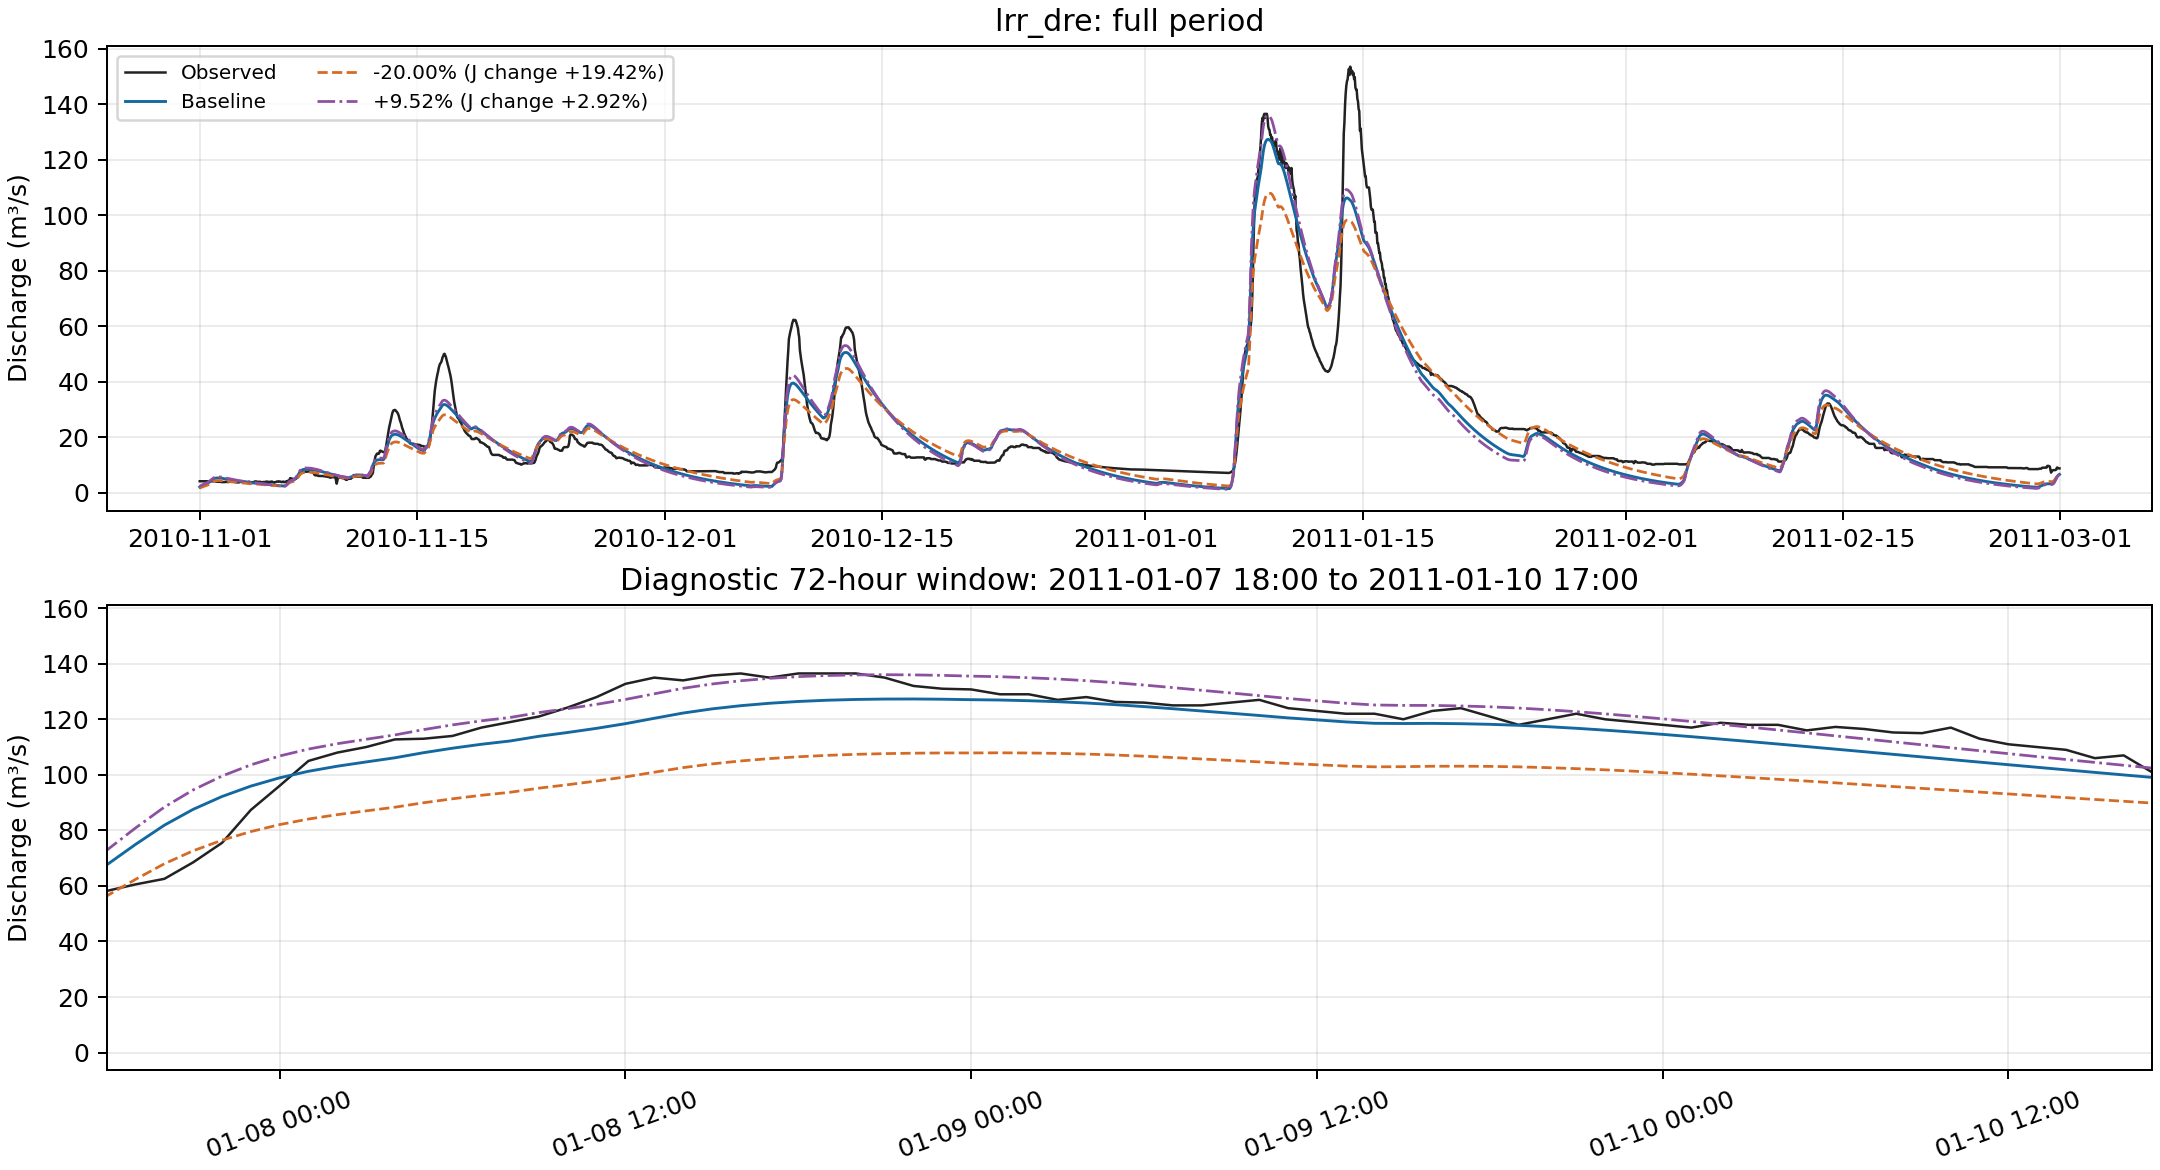
\includegraphics[width=\textwidth]{figures/hydrograph_lrr_dre.png}
\caption{下层水库河道出流系数的流量响应。}
\end{figure}
\param{lrr_dre} 的诊断窗口为 2011 年 1 月 7--10 日。负端扰动在该窗口产生的平方误差净增加量约占全时段净增加量的 82.5\%。正端在此窗口的误差净变化为负，但其全时段目标函数仍增加。上述比例使用带正负号的误差变化计算；正负时段可能抵消，不宜理解为所有误差变化的占比。

这些图支持三个参数能改变流量过程线，并进一步显示影响集中的部分时段；土壤储水、融雪和水库放水的因果路径来自模型方程，还需要结合对应内部状态才能逐事件核实。

\clearpage
\section{加权目标函数的差分进化校准}
将高流量时段最低权重设为 0.7、其他时段最低权重设为 0.1，使用针对原参数附近 60 个扰动点通过最小化最大变化得到的固定权重。以原参数作为初始种群中的一个候选，使用差分进化重新校准；参数边界和随机种子保持不变，关闭原提前收敛停止条件，运行至 700 代上限，共 100944 次目标函数评价。
\begin{center}\begin{tabular}{lrr}\toprule
指标 & 原参数 & 加权校准 700 代\\\midrule
加权目标值 & 0.102420 & 0.099737\\
标准 NSE & 0.907224 & 0.902678\\
观测最大洪峰时刻模拟流量 ($\mathrm{m^3/s}$) & 105.39 & 105.26\\\bottomrule\end{tabular}\end{center}
同一时刻观测为 153.50 $\mathrm{m^3/s}$。此运行因达到预设代数上限而结束，不能标记为自然收敛或全球最优。标准 NSE 和洪峰比较均在校准期内，没有独立验证。
\begin{figure}[H]\centering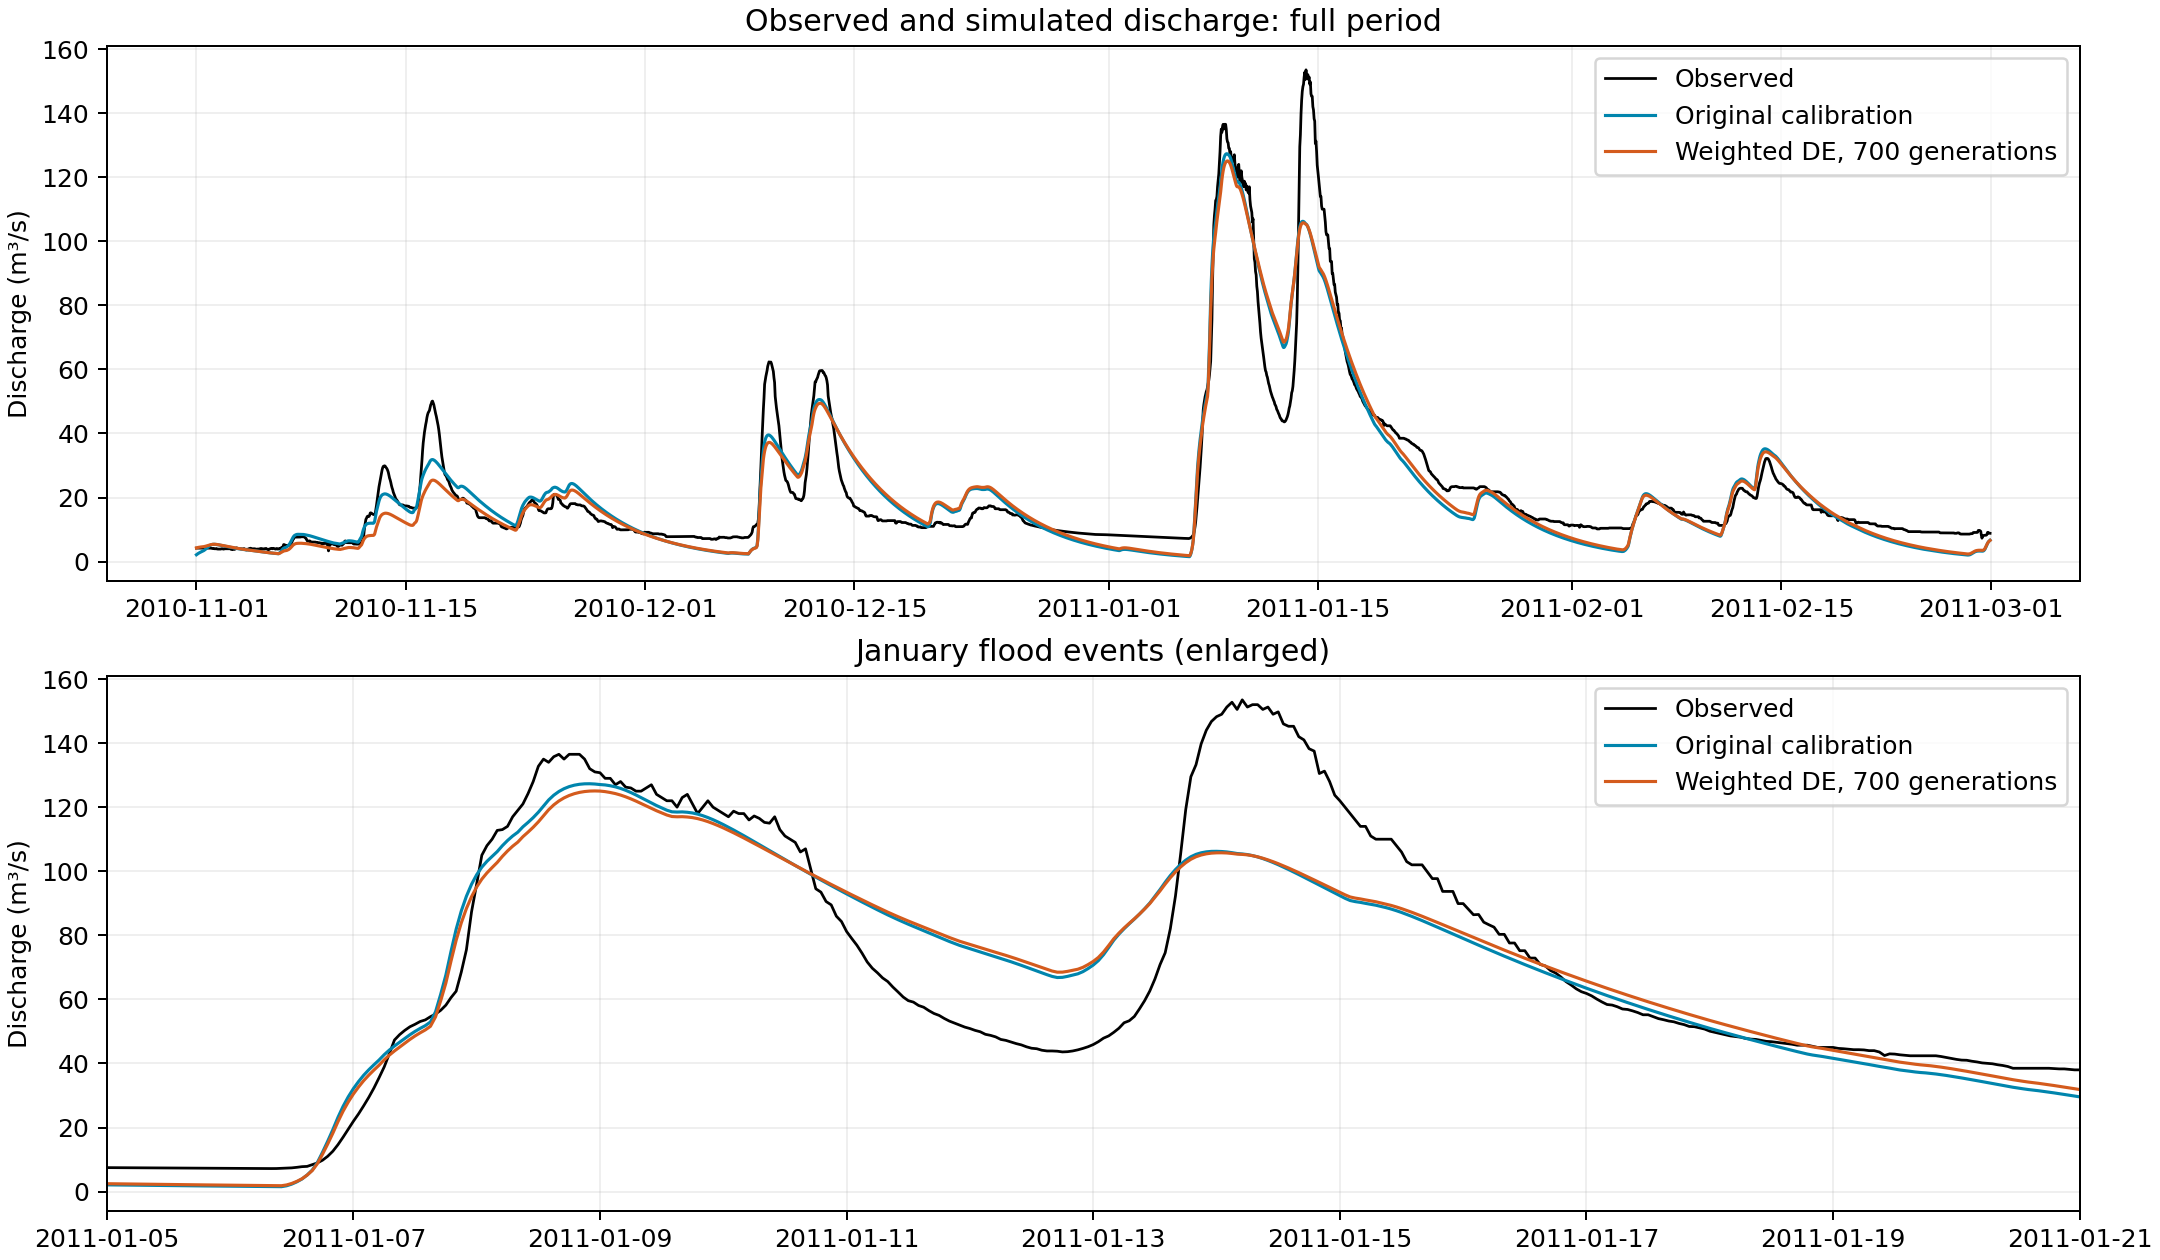
\includegraphics[width=\textwidth]{figures/weighted_de_700_fit.png}\caption{原校准与加权目标函数差分进化校准的流量过程线。}\end{figure}
\clearpage
\subsection{调整前后的敏感性比较}
原实验列使用原参数及 $J=1-\mathrm{NSE}$；加权校准列使用新参数及固定权重的加权目标函数。每列均在对应基准附近逐个扰动，每个参数取 20 个非基准点。平均变化是目标函数绝对相对变化的平均；最大变化是其中最大值。
\begin{center}\small\begin{tabular}{lrrrr}\toprule
参数 & 原平均 & 原最大 & 加权后平均 & 加权后最大\\\midrule
\param{sl0_fcy} & 5.81\% & 16.47\% & 4.63\% & 12.89\%\\
\param{snw_pmf} & 4.77\% & 14.64\% & 4.02\% & 11.96\%\\
\param{lrr_dre} & 4.22\% & 19.42\% & 4.76\% & 16.84\%\\\bottomrule\end{tabular}\end{center}
与原实验相比，三个参数的最大变化均下降，但均未低于 10\%；\param{lrr_dre} 的平均变化反而上升。权重在原基准附近得到的 10\% 限制没有在新基准下保持。权重只针对原扰动点设计，约 31.5\% 时刻接近最低权重；高流量保护也不代表洪峰拟合必然改善。两列使用不同目标函数和参数基准、可行扰动范围也可能不同，因此是各自基准下的相对变化比较，不是标准 NSE 的变化。


\clearpage
\section{绝对误差目标函数重新校准}
将分子和分母都改为绝对值，使用观测均值作为分母参照：
\[J_{\mathrm{abs}}=\frac{\sum_t|Q_t^{\mathrm{sim}}-Q_t^{\mathrm{obs}}|}{\sum_t|Q_t^{\mathrm{obs}}-\overline Q^{\mathrm{obs}}|}.\]
这在所有时刻使用绝对误差，与小误差平方、大误差线性的 Huber 损失不同。差分进化从拉丁超立方随机种群开始，没有将原最佳参数加入初始种群；保留原校准边界，种群倍数 8，随机种子 42，关闭提前停止并运行 700 代，共 100944 次评价。程序因达到代数上限停止，未证明自然收敛或全局最优。
\begin{center}\begin{tabular}{lrr}\toprule
指标 & 原参数 & 绝对误差校准\\\midrule
$J_{\mathrm{abs}}$ & 0.31977 & 0.30188\\
标准 NSE & 0.90722 & 0.87954\\
观测最大洪峰时刻模拟流量 ($\mathrm{m^3/s}$) & 105.39 & 100.60\\\bottomrule\end{tabular}\end{center}
该时刻观测流量为 153.50 $\mathrm{m^3/s}$。新的绝对误差目标值下降，但标准 NSE 降低，最大洪峰时刻的模拟值更低；两者均在校准期计算，未进行独立验证。
\begin{figure}[H]\centering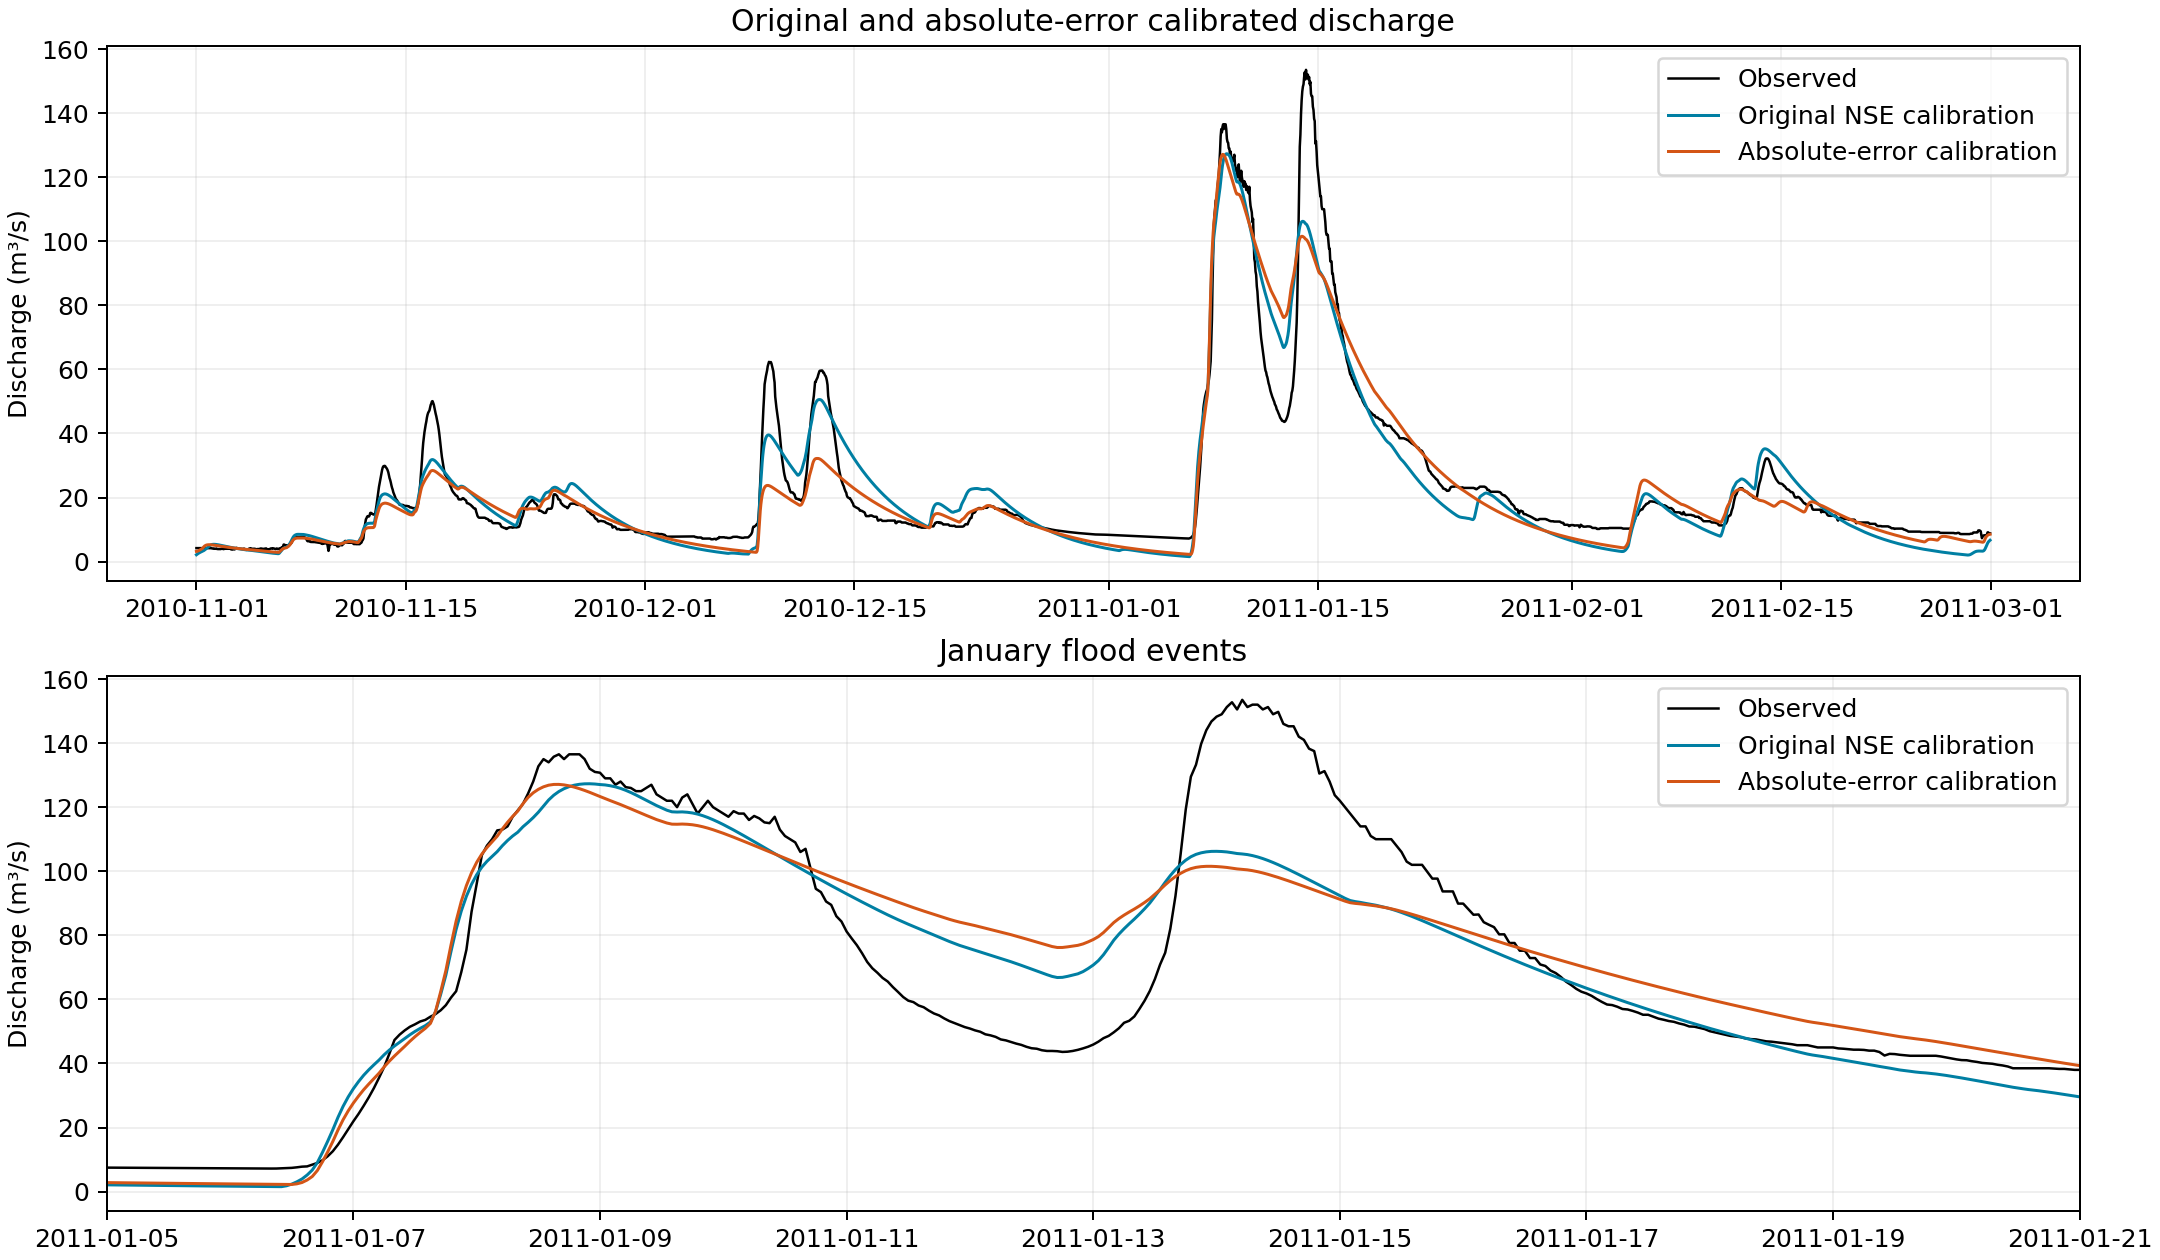
\includegraphics[width=\textwidth]{figures/absolute_de_fit.png}\caption{原 NSE 校准与绝对误差校准的流量过程线。}\end{figure}
\clearpage
\subsection{调整前后的敏感性比较}
原实验列使用原参数及 $J=1-\mathrm{NSE}$；绝对误差列使用新参数及 $J_{\mathrm{abs}}$。两列分别计算各自基准附近 20 个非基准扰动点的平均与最大绝对相对变化。
\begin{center}\small\begin{tabular}{lrrrr}\toprule
参数 & 原平均 & 原最大 & 绝对误差后平均 & 绝对误差后最大\\\midrule
\param{sl0_fcy} & 5.81\% & 16.47\% & 2.18\% & 10.75\%\\
\param{snw_pmf} & 4.77\% & 14.64\% & 1.04\% & 2.80\%\\
\param{lrr_dre} & 4.22\% & 19.42\% & 3.05\% & 10.61\%\\\bottomrule\end{tabular}\end{center}
三个参数的平均和最大相对变化均下降，其中 \param{snw_pmf} 的最大变化低于 10\%；另两个略高于 10\%。两列使用不同目标函数和参数基准，可行扰动范围也可能不同，不能直接视为标准 NSE 的变化。本次没有对全部 18 个参数重新排名。


\section{尚待讨论}
不同随机种子可能产生相近 NSE、但数值差异较大的参数组。当前实验只针对一组已保存的基准参数；更换基准后需要重新检查边界，并评估结论是否稳定。

数据与代码保存在课程目录的 Assignment 2 文件夹。结果表包括单参数扰动表、敏感性排名表和组合扰动表，对应实验脚本也保存在该文件夹中。
\end{document}
